\section{Infrastructure de traitement}\label{sec:rw:sgfd:infra}
La structure interne des systèmes de gestions de flux de données diffère entre les implémentations. Toutefois, plusieurs concepts fondateurs sont couramment utilisés pour permettre l'exécution correcte des requêtes ou pour permettre la gestion des multi-échelles.
\TODO{PLAN}
\subsection{Du modèle vers l'implémentation}
Le modèle théorique permet de savoir la sémantique exacte des expressions de requêtes. La mise en œuvre de ces expressions est plus délicate. La connaissance de cette structure est nécessaire non seulement pour comprendre le fonctionnement des SGFD. Mais de plus, cela permet la mise en œuvre de solutions de médiations de systèmes~\cite{Tatbul:integration}.

\subsubsection{Les résultats intermédiaires}
Comme présenté précédemment en section~\ref{sec:rw:supervision:datastream}, la gestion de flux de données se décompose en trois composants principaux : les sources, les opérateurs et les puits. Les opérateurs consomment une ou plusieurs entités (un flux par exemple) et produisent une nouvelle entité. Ces entités sont matérialisés par des résultats intermédiaires en implémentation comme présenté dans la figure~\ref{fig:rw:sgfd:modeleimplem}.
\begin{figure}[ht]
    \centering
    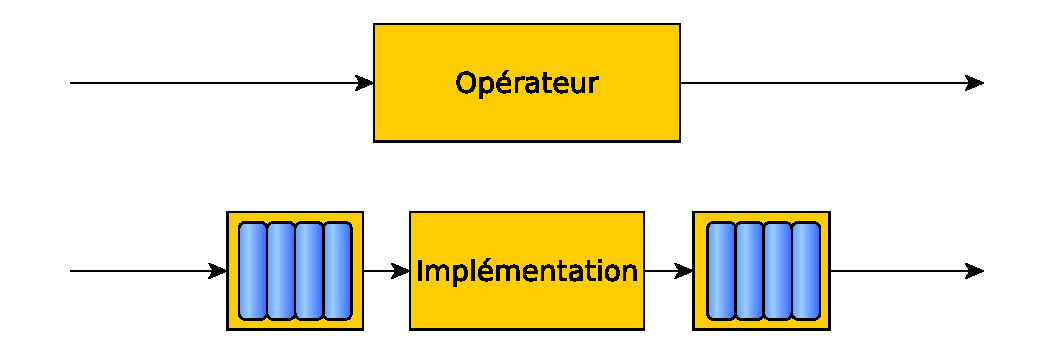
\includegraphics[width=0.8\textwidth]{rw-sgfd-modeleimplem}
    \caption{Implémentation d'un opérateur avec les résultats intermédiaires}\label{fig:rw:sgfd:modeleimplem}
\end{figure}

Ces résultats intermédiaires utilisent des mémoires tampons (et occasionnellement des supports persistants~\cite{Abadi:aurora}). Ces résultats sont manipulé par une interface d'appel très simple en général basé sur les primitives \textit{push} et \textit{pop} tel une pile. Le point crucial de la gestion de flux de données est de maîtriser ces canaux. Leur fonctionnement peut toutefois être plus compliqué en introduisant des primitives d'ordres ou de sélection comme dans les \textit{SweepArea} de \textit{PIPES}~\cite{Kramer:semantics}.

\subsubsection{L'exécution}
Deux types d'exécutions sont référencés : les non-bloquantes et les  bloquantes~\cite{Babcock:issues}. Originellement, un opérateur \textit{bloquant} est \enquote{\it un opérateur qui n'est pas capable de produire son premier n-uplet tant que l'ensemble de son entrée n'a pas été consommé}. Les opérateurs souvent cités sont les agrégats. Par la suite, grâce aux recherches sur les fenêtres~\cite{Maier:semantics}, le terme est généralisé aux opérations de fenêtrages dont le décalage est différent de \textit{1 n-uplet}.

Ainsi, les opérateurs blocants ne sont pas seulement cadencés par le donnée de son entrée. Ils ont leur propre cycle de vie, ce qui les rend bien plus compliqués à exécuter. Le module d'ordonnancement (\textit{scheduler})~\cite{Carney:scheduling} est donc présent dans la plupart des implémentations supportant ce type d'opérateur. Ce composant a pour tâche de décider quel opérateur exécuter et quand.

Quant à la communication entre les canaux et autres modules, les mécanismes de souscriptions (\textit{publish/subscribe} ou \textit{push})~\cite{Eugster:publishsubscribe} ne sont pas toujours adoptés. En effet, au lieu d'appliquer strictement l'approche événementielle, l'infrastructure peut nécessiter de privilégier une approche par appel (\textit{pull}). 

Par exemple, le moteur MXQuery~\cite{Botan:MXQuery} est un SGFD dont la particularité est de traiter des documents \textit{XML} tels que \textit{RSS} (flux d'actualités). Ce moteur ne supporte que l'approche \textit{pull} en entrée. A la différence, un SGFD plus généraliste tel que STREAM supportera un mécanisme événementiel. La gestion de l'hétérogénéité de la dynamique des données s'applique donc aussi au niveau de l'infrastructure d'exécution des requêtes. Pour réussir une médiation de ces mécanismes, il est nécessaire de faire une intégration de systèmes.

\subsubsection{Intégration de systèmes}
Comme nous l'avons présenté, les implémentations de SGFD diffèrent en terme d'architecture, de modèle de requête ou de données, de langage d'implémentation et même de paradigmes d'exécutions. En ce sens, le système Exoengine~\cite{Duller:virtualdsms} virtualise les éléments qui composent un SGFD quelconque. L'implémentation de celui-ci se fait dans le paradigme de programmation à service. Ainsi, les divers canaux exposent deux interfaces de services, l'entrée et la sortie. Il devient désormais possible de relier naturellement des canaux entre eux afin de gérer le flot des données pour les unir ou les disperser vers plusieurs unités de traitement.

\begin{figure}[ht]
    \centering
    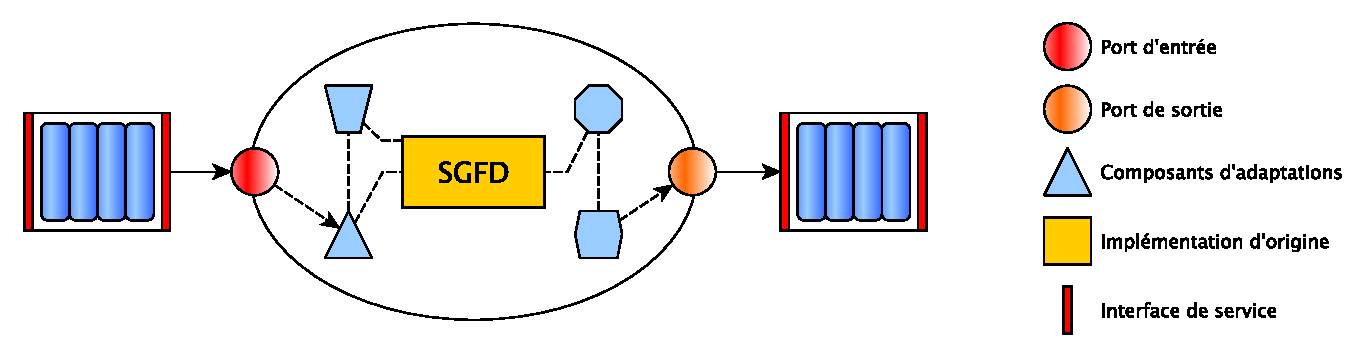
\includegraphics[width=0.8\textwidth]{rw-sgfd-virtualslet}
    \caption{Un \textit{slet} virtuel permettant d'abstraire le fonctionnement d'un SGFD}\label{fig:rw:sgfd:virtualslet}
\end{figure}
Par la suite, il est nécessaire de créer des encapsulations du système originel pour s'adapter à ces interfaces de services. La figure~\ref{fig:rw:sgfd:virtualslet} montre une telle manipulation. La puissance d'une telle approche est non seulement de pouvoir gérer l'hétérogénéité des systèmes, mais aussi de pouvoir :
\begin{itemize}
	\item Rendre un système distribuable. En implémentant des canaux réseaux dont l'entrée est sur une machine et la sortie sur une autre, il devient possible d'avoir une communication entre deux systèmes distribués. L'utilisation du même système sur plusieurs nœuds réseaux permet la distribution du calcul bien que le moteur originel ne le supporte pas.
	\item Convertir un système \textit{pull} en système \textit{push} et inversement. L'hétérogénéité des mécanismes est donc gérée grâce à l'abstraction de service car les canaux supportent les deux modes de fonctionnements.
	\item Utilisation de plusieurs modèles de données. Les canaux transmettent des objets avant tout, celui-ci peut être la représentation d'un \textit{XML} ou d'un n-uplet relationnel. En ajoutant des \textit{slets} de conversions, il est possible de faire fonctionner deux moteurs différents ensemble.
	\item Remplacement d'un composant à chaud. L'utilisation de l'approche à service permet aussi une bonne gestion du cycle de vie des composants. Ainsi, l'administration des requêtes et des composants (\textit{slets} ou canaux) peut se faire pendant que le système est en fonctionnement.
\end{itemize}

Toutefois, la médiation de système n'est valable que d'un point de vue infrastructure. En effet, la mise en œuvre entre les différents systèmes suppose que l'utilisateur est capable de traduire la sémantique de sa requête sur chaque système. Or, nous avons vu qu'il n'existe pas de langage universel permettant de traduire la sémantique de chacun des systèmes pour tous ses aspects.

\subsection{Passage à l'échelle}
L'architecture des SGFD s'est beaucoup concentré sur son passage à l'échelle notamment en terme de volume. En effet, l'intégration des SGFD et des réseaux de capteurs notamment a permit le développement de nouvelles architectures. En effet, les réseaux de capteurs sont capables de se gérer à une portée limité du fait de leur contrainte de puissance et d'énergie. A contrario, les SGFD sont capables de traiter les données sur tout type de plateforme. C'est ainsi que lorsque le nombre de sources s'intensifie que des goulots d'étranglements peuvent se créer et que l'appel aux SGFD devient inévitable.

\subsubsection{Architecture distribué}
La distribution de l'architecture pour passer à l'échelle fait parti des techniques classiques. La structure même des requêtes en forme d'arbre d'opérateur permet la mise en œuvre naturelle de structures hiérarchiques. En effet, des systèmes tels que \textit{Borealis}~\cite{Abadi:borealis} (historiquement, l'évolution d'\textit{Aurora}) permettent de distribuer le calcul d'une requête sur plusieurs nœuds avec toutes les complications que cela implique.

La distribution d'un calcul emmene les problématiques de synchronisation, de répartition de charge, des tolérances aux fautes, etc... Des recherches~\cite{Hwang:distributed, Tucker:heartbeat} ont donc été faites sur ce point pour permettre une évaluation exacte avec une latence faible pour garantir un traitement rapide.

L'approche hiérarchique permet de faire du traitement à plusieurs niveaux. Ces niveaux peuvent avoir un rôle bien défini dans le traitement des données. C'est le cas pour \textit{HiFi}~\cite{Franklin:hifi} présentant cinq niveaux de traitement des données. À chaque niveau correspond un type d'opération et à une localisation bien défini :
\begin{itemize}
	\item[\textbf{Nettoyage} :] Application de filtres sur les données pour enlever les anomalies. Traitement situé sur le capteur.
	\item[\textbf{Lissage} :] Interpolation des mesures perdues. Utilisation d'agrégats sur les fenêtres. Traitement situé sur la station d'accueil des capteurs.
	\item[\textbf{Arbitrage} :] Consolidation des données. Suppression de données dupliquées, agrégations des données nécessaires au niveau suivant. Traitement situé au niveau d'un batiment.
	\item[\textbf{Validation} :] Applications de règles métiers pour valider les données. Utilisation principale de jointures. Traitement situé à un niveau régional.
	\item[\textbf{Analyse} :] Support de décisions tels que vu dans la section~\ref{sec:rw:supervision:warehouse}. Traitement situé au centre de commandement.
\end{itemize}

Cette approche a été généralisé dans \textit{SStreamWare}~\cite{Gurgen:sstreamware} avec les \textit{sites de contrôles} (plus haut niveau hiérarchique) et les \textit{passerelles}. Ces dernières sont capables d'accueillir des capteurs (virtuels ou non), ainsi que d'exécuter une requête de flux sur les capteurs accueillis ou sur des flux externes venant d'une autre passerelle. Le site de contrôle est celui qui distribuera la requête sur les différentes passerelles.

\subsubsection{Désignation}\label{sec:rw:sgfd:infra:designation}
Plus le nombre de sources augmente, plus il devient difficile de maîtriser lesquels sont concernés par la requête que l'utilisateur souhaite déployer. Une requête par désignation est une requête utilisant une autre requête pour désigner les sources de données à lire. Par exemple : \enquote{\it Le flux des mesures des capteurs de température du batiment A}. Dans cette requête, il est nécessaire de d'abord faire une interrogation sur l'expression \enquote{\it Quels sont les capteurs situés dans le batiment \textit{A} et de type \textit{température}} avant de déployer la requête.

Ce procédé est naturellement implanté dans notamment SStreamWare, HiFi et GSN~\cite{Aberer:gsn}. L’objectif à long terme de ce dernier est de former un internet de capteur. Son architecture est donc naturellement pair-à-pair. L’interrogation continue sur ce système peut se faire par le déploiement d’un nouveau capteur virtuel. La désignation est donc centrale, car la formation d’un capteur virtuel à partir d’autres sources est possible. Toutefois, du fait de l’absence de méta-données la puissance d'expression de cette requête de désignation est limité. Dans SStreamWare et HiFi, au contraire, le support des méta-données telles que son lieu, son type ou sa fréquence d'émission permet de correctement sélectionner les sources concernés.

\subsection{Synthèse}
L'infrastructure des SGFD a reçu beaucoup d'attention en terme d'architecture, de tolérance aux fautes, d'intégration et de support des multi-échelles. Le point crucial manquant reste encore la compréhension de la sémantique des requêtes. En effet, lors de l'intégration des systèmes, qui est la pierre angulaire de la compréhension des infrastructures, nous avons vu qu'il était nécessaire que l'utilisateur sache traduire l'expression de ses sous-requêtes dans les différents langages. De plus, du fait de l'ambiguïté sémantique de l'exécution des différents opérateurs tels que nous l'avons décrite dans la section~\ref{sec:rw:sgfd:modeles}, l'expression de ces requêtes peut porter à confusion. De façon similaire, le procédé de désignation semble limité en pouvoir d'expression. Son exécution, en terme d'infrastructure, est limité car, par définition, l'exécution d'une requête en implique une autre avant son déploiement. Une généralisation de cette approche est donc nécessaire.